
\subsection{Frontend}

The web interface is built around the Angular Framework and is programmed in TypeScript and HTML.
Angular is designed around components and services. 
The components consist of HTML and CSS to define how the component is rendered and typescript class which defines the behaviour of the component. 
A component can be instantiated in other components to build the user facing webpage. 
Services provide global functionality and a service can be injected into any given component providing access to the properties and methods of the service. 
Using Angular directives components can be dynamically generated depending on the data as defined by their class. 
For example, the *ngFor directive will duplicate a template of HTML for each iteration of the for loop.

\subsubsection*{Overview}
The web interface is built around the Angular Framework and is programmed in TypeScript 
and HTML. The back end server hosts the web interface and the rover is controlled through the API
that the backend exposes.

\subsubsection*{Features}
The webpage consists of 3 tabs, a dashboard, a console log and a settings panel. 
The dashboard is broken into 4 sub panels.
\begin{itemize}
    \item Map
    \item 3D Viewport
    \item Telemetry
    \item Control Panel
\end{itemize}

\newpage
\begin{wrapfigure}{l}{0.5\textwidth}
    \centerline{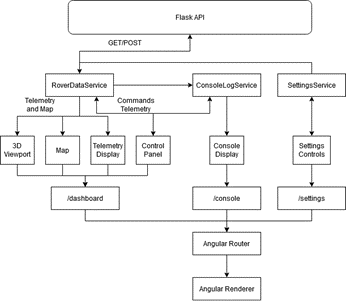
\includegraphics[width=0.45\textwidth]{images/frontend-flow.png}}
    \caption{Frontend design overview}
\end{wrapfigure}

There are 3 services running in the background which maintain the information that is rendered. 
The rover data service maintains the connection to the server, 
the console logging service provides interfaces for adding to the log and events for when a new entry is added and the settings service maintains a global settings object which can be modified by a component and also provides an event for when that has happened.
The Angular router is a system to dynamically update the DOM based on the URL in the client browser without hosting separate web pages on the server. This enables the production of single page applications (SPAs) and can dynamically load components from the server based on the URL in the browser without changing the URL from the server’s perspective.~\cite{ref:angular_router}

\subsubsection*{Map Display}
The map display is a 2D representation of the segway's internal map. The map is updated in real time as the segway explores the environment and identifies features. The map is rendered using Two.js as it is a simple and lightweight library that allows for easy rendering of shapes. It is designed for modern browsers and can render to multiple systems, WebGL, Canvas or by drawing native SVG shapes.~\cite{ref:twojs} The map is rendered as a series of lines representing the walls and connections between nodes on of the maze

\subsubsection*{3D Viewport}
The 3D viewport displays a 3D model of the segway that is updated with the tilt and orientation of the segway from the telemetry service. It is rendered with Three.js, again as it is an easy to use library that is relatively lightweight.~\cite{ref:threejs}

\subsubsection*{Telemetry Display}
The telemetry panel displays the current state of the rover. This includes the current position, orientation, state, and a feed from the sensors

\subsubsection*{Control Panel}
The control panel is a set of buttons that allow the user to send commands to the segway manually. As the segway is autonomous this is a START/STOP button that allows the user to start and stop the segway's autonomous exploration. There is also a toggle to enable auto-updating of the telemetry and map data.

\subsubsection*{Console Display}
The console displays a log of events, warnings and errors that are generated by both the front-end and the segway itself. These are stored in the ConsoleLogService. This is useful for debugging and monitoring the segway's state.

\subsubsection*{Settings Display}
The settings display provides a simple interface to modify an internal state of settings.

\subsubsection*{Rover Data Service}
The rover data service uses the Angular http client to make GET requests to the server. The responses from the server are instantiated as an interface. The design of the interfaces matches the data returned from the API. The service has an interval timer which calls an update function every 200ms by default which constantly overwrites the internal data store. When this happens an EventEmitter is triggered which a component can subscribe to so that it is informed when the latest telemetry is available. A similar process is followed for the map data.
An example of one of the interfaces is shown in figure \ref{code:telemetry_interface}.

\begin{figure}
    \begin{minted}{typescript}
export interface Telemetry{
    id:number;
    position:Position;
    accelerometer:xyzValue;
    gyroscope:xyzValue;
    steps:number,
    state:"start"|"stop"|"mapping"|"solving"|"error"
}
    \end{minted}
    \caption{The telemetry interface}
    \label{code:telemetry_interface}
\end{figure}

\subsubsection*{Implementation}
Each panel is implemented as a separate component in Angular. The components are then combined into a single page application using the Angular router.
The telemetry is backed by a service that polls the server and maintains an internal telemetry state, matching with the latest telemetry sent from the rover.
The console is backed by another service that stores the log events and provides EventEmitters for new log events.

\subsubsection*{Design}
The design of the interface is based on the Material Design specification. This is a design language developed by Google. The components are provided by the Angular Material package which 
provides a set of components such as buttons, input panels and menu elements. All of which follow the Material Design specification.~\cite{ref:angular_material}

% Image of frontend

\subsubsection*{Testing}
Angular provides a unit testing system using spec files to define the intended behaviour of a given component. When running then ng test command each component is instantiated and properties of the component is compared against the specification defined in the .spec file.

\subsubsection*{Further Goals}
The implementation of an authentication system would have been ideal 
as currently any client can access the information of any segway and
there is no verification that the information sent form the segway is
truly from the device you are using. This could be done using authentication tokens
handed out by the server. When a segway is onboarded to the server
it responds with a randomly generated token which will be sent 
over HTTPS. A similar process for the client, this way each API
call must have the associated token to be accepted. 
An account-based log-in system could authenticate the client 
and give them control over a limited number of segways for example.